%\documentclass[twocolumn]{article}
%\usepackage[utf8]{inputenc}
%\documentclass[10pt,journal,onecolumn]{IEEEtran}
%\documentclass[10pt,journal,compsoc]{IEEEtran}
\documentclass[10pt, journal, letterpaper]{IEEEtran}


% NB hyperref package may need to be commented for Latex upload
\usepackage{cite}

%important package
\usepackage{multirow} 
\usepackage{algpseudocode}
\usepackage{algorithm}
\usepackage{rotating}
\usepackage{kantlipsum} %with the next two command (commath, allowdisplaybreaks) -> allow to break the formulas along the pages
\usepackage{commath}
\allowdisplaybreaks
\usepackage{mathtools}  %with the next command adjust the vertical space between formulas
%\setlength{\jot}{5pt}
%\usepackage{ragged2e}   %if add \justify at each line, that line would be justified. This is used because the abstract of transaction style is not justified  ---- it is not compatible with twocolumn-IEEETrans
%not important
\usepackage{verbatim}
\usepackage{xr-hyper} 
\usepackage{enumitem}
\usepackage{multirow}
\usepackage[table,xcdraw]{xcolor}
\usepackage{array,arydshln}
\usepackage{graphicx,booktabs}
\usepackage{longtable}
%strikethrough not working when nested in a definition
%\usepackage[normalem]{ulem}
%\usepackage{soul}
%\usepackage{fullpage} 
%%%%%%%%%%%%%%%%%%%%%%%%%%%%%%%%%%%%%%%%%%%%%%%%%%%%%%%%%%%%%%%%%%%%%%%%%%%%%
% hyperref package may need to be commented for Latex upload
%\usepackage[pdfusetitle, pdfauthor={Michael Shell, My institution}]{hyperref}
%%%%%%%%%%%%%%%%%%%%%%%%%%%%%%%%%%%%%%%%%%%%%%%%%%%%%%%%%%%%%%%%%%%%%%%%%%%%%
\usepackage{balance}
\usepackage{flushend}
\usepackage{epstopdf}
\usepackage{wrapfig}
\usepackage{latexsym}
\usepackage{amssymb}
\usepackage{amsthm}
\usepackage{amsfonts}
\usepackage{amsmath} %[cmex10]
%\usepackage{flushend} %********************* This package has a bug: Do no include it
\usepackage{graphicx}
\usepackage{latexsym}
\usepackage{booktabs}
\usepackage[style=base]{caption}
\usepackage{subcaption} %******************* This package has conflict with sufig and subfigure
%\usepackage{subfigure}
%\usepackage{subfig}
\usepackage{breqn}
\newtheorem{thm}{Property}
\newtheorem{thm1}{Theorem}
\newtheorem{thm3}{Proposition}
\newtheorem{thm5}{Remark}
\newtheorem{thm7}{Lemma}
\algnewcommand\algorithmicinput{\textbf{INPUT:}}
\algnewcommand\INPUT{\item[\algorithmicinput]}
\algnewcommand\algorithmicoutput{\textbf{OUTPUT:}}
\algnewcommand\OUTPUT{\item[\algorithmicoutput]}
\usepackage[table]{xcolor}
%\usepackage[dvipsnames]{xcolor}
%\usepackage[cmyk]{xcolor}
%\usepackage{natbib}
\usepackage{graphicx}
\usepackage{mathtools}
\usepackage{enumitem,kantlipsum}
\usepackage{adjustbox}
% change the width and height of rows and columns in Tables
\usepackage[thinlines]{easytable}

\algdef{SE}[DOWHILE]{Do}{doWhile}{\algorithmicdo}[1]{\algorithmicwhile\ #1}
\makeatletter
\algnewcommand{\LineComment}[1]{\Statex \hskip\ALG@thistlm \texttt{#1}}
\makeatother
\newcommand{\export}{Exportation\xspace}
\newcommand{\move}{Move\xspace}
\newcommand{\ouralgorithm}{GPE\xspace} %%Green path exportation

\newlength\mylength
\setlength\mylength{\dimexpr.13\columnwidth-1\tabcolsep-0.2\arrayrulewidth\relax}
\usepackage{color}
% we need a better fix for this, see https://tex.stackexchange.com/questions/64298/error-with-xcolor-package
\colorlet{BLUE}{blue}
\usepackage{colortbl}
\definecolor{LightCyan}{RGB}{155, 227, 247}

%\newcommand{\optional}[1]{#1}
%\newcommand{\optional}[1]{\textcolor{Orange}{#1}}
\newcommand{\optional}[1]{\ignorespaces}


\newif\ifrevisionactive
\newif\ifshowdeleted
\revisionactivetrue
%\showdeletedtrue

\newcommand{\revised}[1]{\ifrevisionactive \textcolor{blue}{#1} \else \textcolor{black}{#1} \fi}

%\newcommand{\deleted}[1]{\ifrevisionactive \ifshowdeleted \textcolor{red}{\sout{#1}} \else \fi \fi}
\newcommand{\deleted}[1]{\ifrevisionactive \ifshowdeleted \textcolor{orange}{#1} \else \fi \fi}


% correct bad hyphenation here
\hyphenation{net-works mo-ni-to-ring par-ti-cu-lar pe-ri-o-di-cal-ly mi-ni-mi-zing va-ria-tions de-li-ve-red per-ri-o-di-cal-ly}


\newcommand\linearFigSze{0.48}
\newcommand\histFigSze{0.48}
\newcommand\boxFigSze{1}

\newcommand{\red}[1]{\textcolor{red}{#1}}

\newcommand\figSzeMahdi{0.8}

\begin{document}
\title{GEANT: Traffic Pattern, Break Down to Elements, and COVID-19 impacts}
\author{}
%\date{October 2018}
\maketitle	
\begin{abstract}
In this paper, the impact of weekends, new year holidays, and COVID-19 pandemic on GEANT network traffic is investigated. Our observation shows that 
\end{abstract}	
\begin{IEEEkeywords} 
    Passive Network Monitoring, Traffic Break-Down, New Year Holidays Impact, Covid-19 Impact;
\end{IEEEkeywords}

\section{Introduction}
INTRODUCTION TO GEANT.

DATA-SET WE USED.

A BRIEF POINT TO OUR FINDINGS.

\section{Impact of weekends on GEANT}
In this section, we compare the traffic pattern during working days and weekends. To this end, we observe network traffic for fifteen weeks. On every day, the average traffic per hour is collected and the median of all data collected during these fifteen weeks is considered as the Representative. To remove the impact of special event, e.g., Christmas and new year holidays, non-consecutive weeks are selected. The investigated dates are 2019/11/04 - 2019/12/22 and 2020/01/20 - 2020/03/22.

\subsection{Total Traffic Throughput}
If Fig.~\ref{fig:OW_bps_fps}, the impact of weekends on the traffic pattern is illustrated. Fig.~\ref{fig:OW_bps} shows median of data-rate during fifteen different weeks. Based on our observation, has a significant reduction at weekends. On the other hand, during working days, there is a mild change in data-rate. Starting from Monday, it has an smooth increasing trend until Wednesday where the highest amount of data-rate is reported on. Starting from Wednesday, there is an smooth decreasing trend until Friday. In total, data-rate during Monday to Thursday are next to each other while they are slightly higher than Friday.
\begin{figure}[!htb]
\centering
    \begin{subfigure}{\figSzeMahdi\columnwidth}
          \centering
          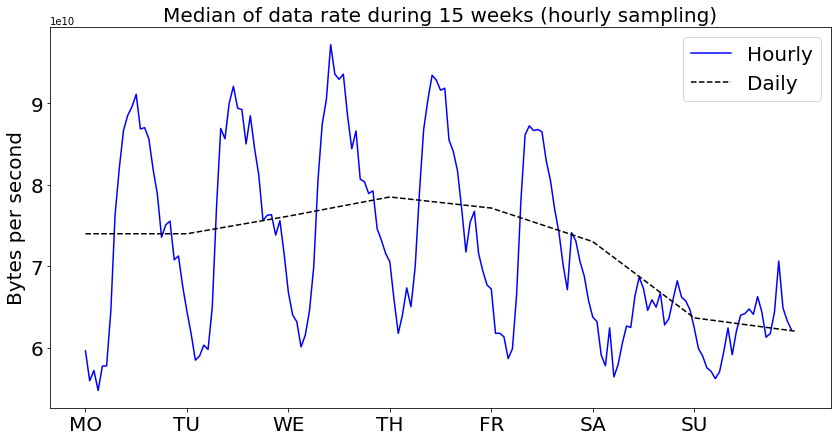
\includegraphics[width=\columnwidth]{img/OW_byterate.png}
          \caption{Data-rate}
          \label{fig:OW_bps}
    \end{subfigure}
    \begin{subfigure}{\figSzeMahdi\columnwidth}
          \centering
          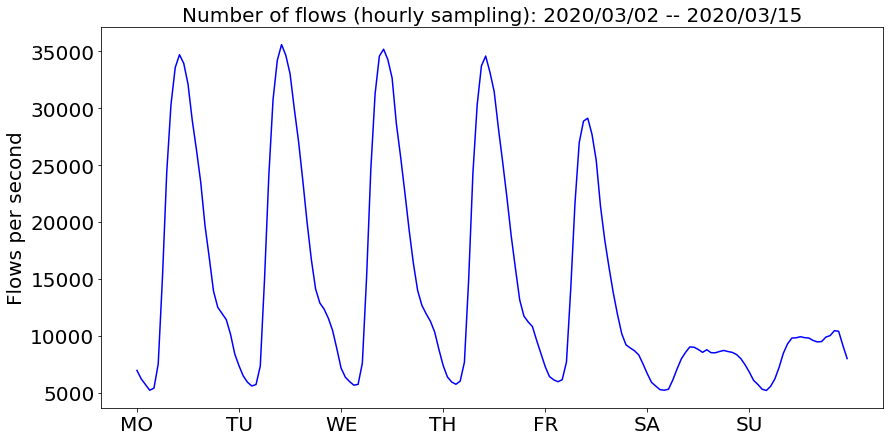
\includegraphics[width=\columnwidth]{img/OW_flowrate.png}
          \caption{Flow-rate}
          \label{fig:OW_fps}
    \end{subfigure}
    \caption{Median of observed traffic pattern during 15 weeks}
    \label{fig:OW_bps_fps}
\end{figure}

Fig.~\ref{fig:OW_fps} represented the number of flows in the network. Our data shows that the number of observed flows is approximately the same during the first four working days. However, there is a mentionable decrease in the reported flow-rate on Friday which may be interpreted as people getting ready for weekends.

\subsection{Academic and Business Traffic}
In Fig.~\ref{fig:OW_acaBus_bps_fps}, the academic and business components of GEANT network traffic are plotted separately to have a better understanding of the network traffic pattern.
\begin{figure}[!htb]
\centering
    \begin{subfigure}{\figSzeMahdi\columnwidth}
          \centering
          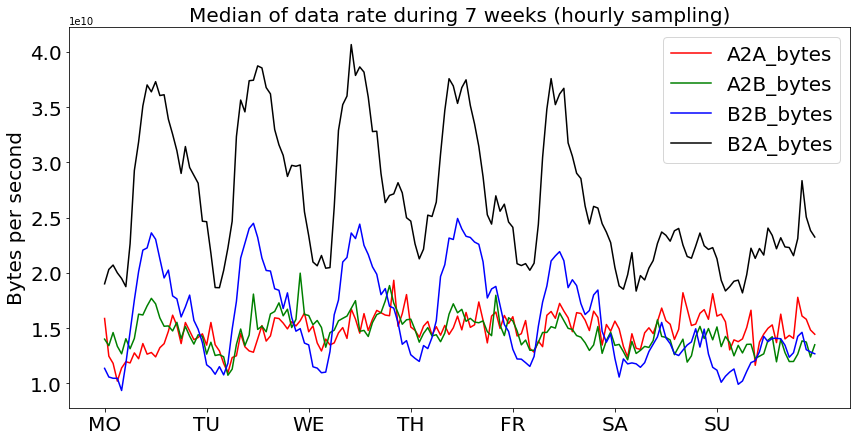
\includegraphics[width=\columnwidth]{img/BCH_acaBus_bps.png}
          \caption{Data-rate}
          \label{fig:OW_acaBus_bps}
    \end{subfigure}
    \begin{subfigure}{\figSzeMahdi\columnwidth}
          \centering
          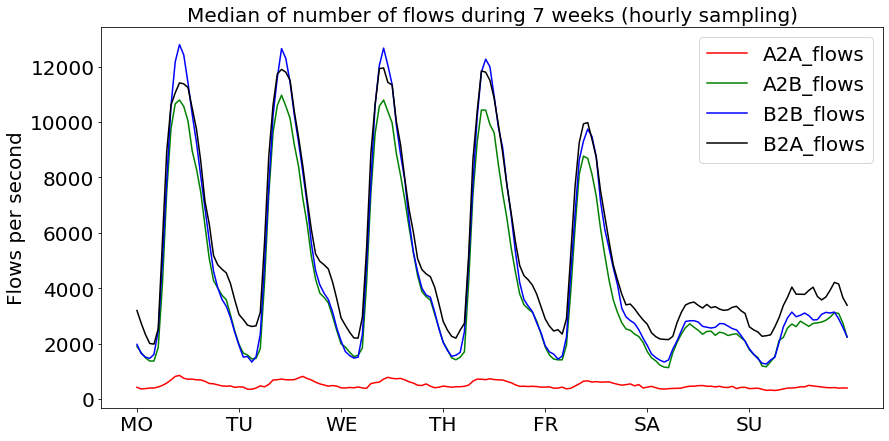
\includegraphics[width=\columnwidth]{img/BCH_acaBus_fps.png}
          \caption{Flow-rate}
          \label{fig:OW_acaBus_fps}
    \end{subfigure}
    \caption{Median of observed traffic pattern during 15 weeks}
    \label{fig:OW_acaBus_bps_fps}
\end{figure}
Considering the data-rate during working days, those flows originating from business ASes (we call these flows 'business traffic') are patterned and consequently more predictable. The data conveyed through these flows usually starts to rise in the morning and reaches its highest amount at noon. At the weekend, not only the overall date-rate of business traffic decreases significantly but also the pattern changes. During the weekend, the traffic data-rate starts to rise a bit later than working days. Besides, when data-rate reaches its maximum it stays their for a longer period of time. Consequently, a huge delay is applied to the time when the data-rate starts to fall comparing with working days.
Throughout the rest of this paper, those flows originating from academic ASes are called academic traffic. Academic traffic has similar behaviour during the working days and weekend, especially, those that are destined to an academic AS as well. 

Fig.~\ref{fig:OW_acaBus_fps} presents the number of flows traversing GEANT network per second. Interestingly, those academic flows that are destined to business ASes show a different behaviour comparing to their data-rate pattern. Similar to business traffic, academic to business traffic has a clear pattern in working days: start to rise in the morning, hit the max at noon, and fall later on. At weekend, not only flow-rate decreases significantly but also it stays at its peak for a longer period of time. On the other hand, academic to academic traffic (traffic originated and destined from/to academic ASes) has a very low flow-rate comparing to the other types of traffic. Considering this along with the data-rate (Fig.~\ref{fig:OW_acaBus_bps}), we can infer that in average, the size of flows in academic to academic traffic is bigger than the other types of traffic (it has a very low flow-rate but a mentionable data-rate). Similarly, the average size of academic to business flows is lower than the others. Comparing business to academic and business to business traffic, the average size of the first one is higher than the later one.

\subsection{Top ASes}
Fig.~\ref{fig:topAS_bps_OWD_OWE} compares the data-rate of the top 7 ASes during working days and weekend. In order to specify the top 7 ASes generating data, the summation of data traffic generated by different ASes over the ordinary week is calculated. Thereafter, the ASes corresponding to the top 7 values are selected as the top 7 ASes generating data traffic during the ordinary week. The same computation is carried out to find the top 7 ASes generating/receiving flow and receiving data traffic. Fig.~\ref{fig:OWE_topAS_bps} shows the top 7 ASes during working days of the ordinary week while Fig.~\ref{fig:OWE_topAS_bps} focuses on weekend days. 

\begin{figure}[hbt!]
    \centering
    \begin{subfigure}{\columnwidth}
          \centering
          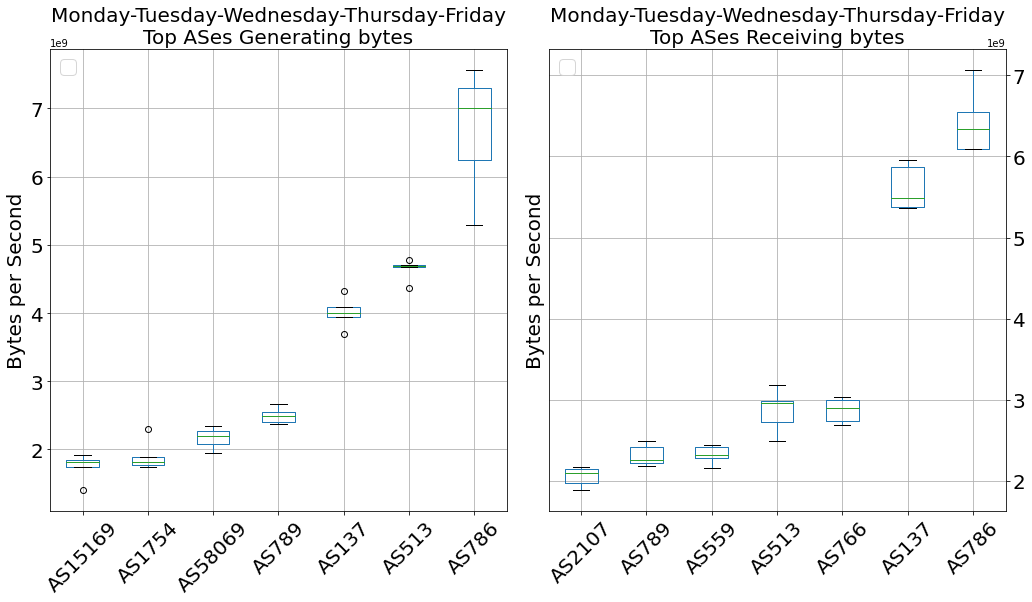
\includegraphics[width=\columnwidth]{img/OWD_top7ASes_bps.png}
          \caption{Data-rate during working days}
          \label{fig:OWD_topAS_bps}
    \end{subfigure}
    \begin{subfigure}{\columnwidth}
          \centering
          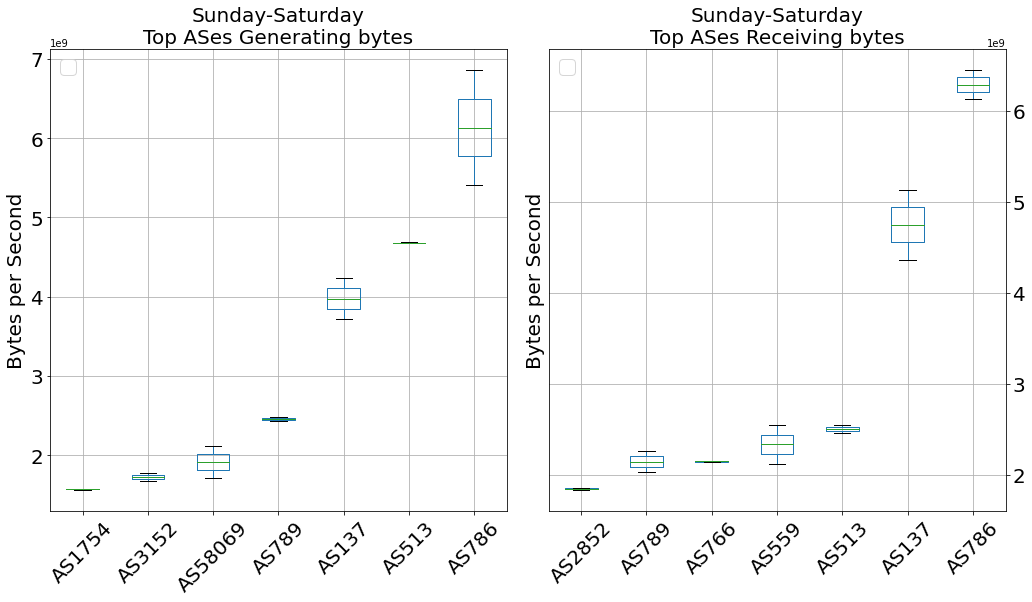
\includegraphics[width=\columnwidth]{img/OWE_top7ASes_bps.png}
          \caption{Data-rate during weekends}
          \label{fig:OWE_topAS_bps}
    \end{subfigure}
    \caption{Impact of weekends on data-rate of top 7 ASes}
    \label{fig:topAS_bps_OWD_OWE}
\end{figure}
Our data shows that not only the top 3 ASes generating data are the same during working and weekend days but also they are generating almost the same amount of traffic. Although we do not have supporting evidence, we believe this is a lead that the majority of traffic in these ASes falls into the machine to machine category. Surprisingly, these top 3 ASes generating data are the same as the top 3 ASes receiving traffic.  Table~\ref{tab:OWD_OWE_ASMap} maps the AS number to corresponding name. 
\begin{table}[h!]
	\caption{Map AS number to AS name.}
	\label{tab:OWD_OWE_ASMap}
	\centering
	%	\begin{center}\small
	\resizebox{\columnwidth}{!}{%
	%\tiny
	\begin{tabular}{|c||l|} 
		\hline
		\textbf{AS Number} & \textbf{Description}\\
		\hline\hline
		$AS786$ & JANET Jisc (UK NREN)  \\\hline
		$AS137$ & GARR (Italian NREN)  \\\hline
		$AS513$ & CERN (European Nuclear Research) \\\hline
		$AS766$ & RedIRIS (Spain NREN) \\\hline
		$AS559$ & SWITCH (Switzerland Innovation Corporation)  \\\hline
		$AS789$ & IN2P3 IN2P3 (French Nuclear $\&$ Particle Research)  \\\hline
		$AS2107$ & ARNES-NET (Slovenia NREN)  \\\hline
		$AS58069$ & KIT-GRIDKA (German Nuclear Research) \\\hline
		$AS1754$ & DESY-HAMBURG (German Particle Research) \\\hline
		$AS15169$ & GOOGLE, US \\\hline
		$AS2852$ & CESNET2 (Czech NREN)\\\hline
		$AS3152$ & FNAL (US Particle Physics Research) \\\hline
		$AS32934$ & FACEBOOK, US\\\hline
		$AS1955$ & HBONE KIFU (Hungarian ISP)\\\hline
		$AS378$ & MACHBA ILAN (Israelian NREN) \\\hline
		$AS2108$ & CARNET (Croatian NREN) \\\hline
		$AS16509$ & AMAZON-02, US \\\hline
		$AS5408$ & GRNET (Greek NREN)\\\hline
		$AS202425$ & INT-NETWORK, SC\\\hline
		$AS49505$ & SELECTEL (Russian Internet hosting provider) \\\hline
    \end{tabular}}
    	%	\end{center}
\end{table}
In order to have a simpler comparison between the rank of top 7 ASes in generating and receiving traffic, Table~\ref{tab:OWD_OWE_ASRank_bps} is provided. For example, all four entries for Jisc are one, meaning that Jisc is the top AS I. generating data during working days, II. receiving data during working days, III. generating data during Week Ends, and IV. receiving data during weekends. On the other, FNAL is not among the top 7 ASes during working days, however, it is the sixth AS generating data during weekend days.
\begin{table}[h!]
	\caption{Rank of Top ASes Generating (Gen.) or Receiving (Rec.) \textbf{data} during Working Days (WD) and WeekEnd days (WE).}
	\label{tab:OWD_OWE_ASRank_bps}
	\centering
	%	\begin{center}\small
	\resizebox{\columnwidth}{!}{%
	%\tiny
	\begin{tabular}{|l||c|c|c|c|} 
		\hline
		\textbf{AS Number} & \textbf{WD Gen.} & \textbf{WD Rec.}& \textbf{WE Gen.}& \textbf{WE Rec.}\\
		\hline\hline
		$AS786$ (Jisc) & 1 & 1 & 1 & 1  \\\hline
		$AS137$ (GARR) & 3 & 2 & 3 & 2 \\\hline
		$AS513$ (CERN) *& 2 & 3 & 2 & 3 \\\hline
		$AS789$ (IN2P3) *& 4 & 6 & 4 & 6\\\hline
		$AS766$ (RedIRIS) & - & 4 & - & 5 \\\hline
		$AS559$ (SWITCH) & - & 5 & - & 4 \\\hline
		$AS58069$ (GRIDKA) *& 5 & - & 5 & -\\\hline
		$AS1754$ (DESY) *& 6 & - & 7 & - \\\hline
		$AS15169$ (Google) & 7 & - & - & - \\\hline
		$AS2107$ (ARNES) & - & 7 & - & - \\\hline
		$AS3152$ (FNAL) +& - & - & 6 & -\\\hline
		$AS2852$ (CESNET2) & - & - & - & 7\\\hline\hline
		\multicolumn{2}{|c|}{\textbf{Gen. = Generating}} & \multicolumn{3}{||c|}{\textbf{Rec. = Receiving}} \\\hline\hline
		\multicolumn{2}{|c|}{\textbf{WD = Working Days}} & \multicolumn{3}{||c|}{\textbf{WE = WeekEnd days}} \\\hline\hline
		\multicolumn{2}{|l|}{*: EU Nuclear or Particle Physic Related} & \multicolumn{3}{||c|}{+: US Nuclear or Particle Physic Related} \\\hline
    \end{tabular}}
    	%	\end{center}
\end{table}

In Fig.~\ref{fig:topAS_fps_OWD_OWE}, top 7 ASes with respect to incoming and outgoing flow-rate is depicted. Contrary to data-rate, the top flow-rates during working and weekends are dramatically reduced.
\begin{figure}[h!]
    \centering
    \begin{subfigure}{\columnwidth}
          \centering
          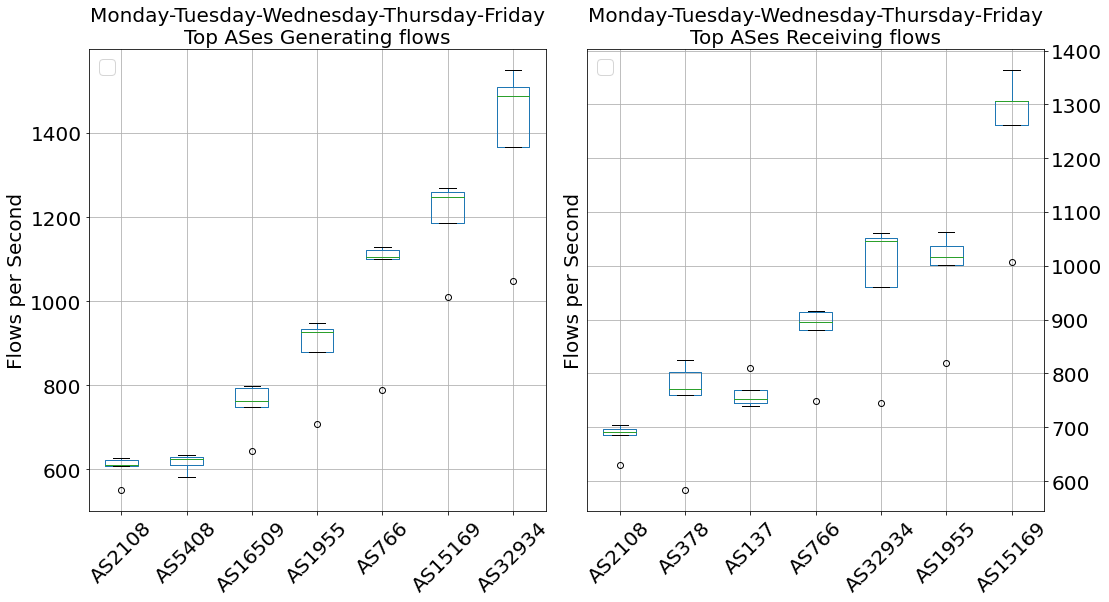
\includegraphics[width=\columnwidth]{img/OWD_top7ASes_fps.png}
          \caption{Flow-rate during working days}
          \label{fig:OWD_topAS_fps}
    \end{subfigure}
    \begin{subfigure}{\columnwidth}
          \centering
          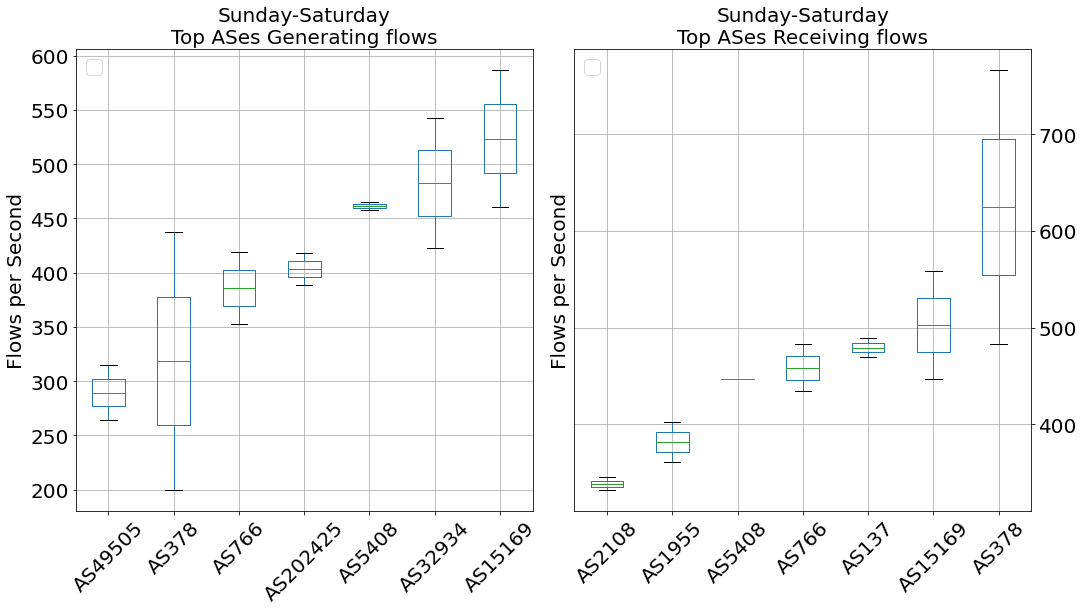
\includegraphics[width=\columnwidth]{img/OWE_top7ASes_fps.png}
          \caption{Flow-rate during weekends}
          \label{fig:OWE_topAS_fps}
    \end{subfigure}
    \caption{Impact of weekends on flow-rate of top 7 ASes}
    \label{fig:topAS_fps_OWD_OWE}
\end{figure}
Although Google and Facebook are not among top 6 ASes\footnote{Google is the 7th data generator during working days.} generating or receiving data, they are first and second flow generator and receiver during working days. Interestingly, Facebook is not among top 7 ASes in terms of number of received flows while it has the second rank of receiving number of flows during weekends.
\begin{table}[h!]
	\caption{Rank of Top ASes Generating (Gen.) or Receiving (Rec.) \textbf{flow} during Working Days (WD) and WeekEnd days (WE).}
	\label{tab:OWD_OWE_ASRank_fps}
	\centering
	%	\begin{center}\small
	\resizebox{\columnwidth}{!}{%
	%\tiny
	\begin{tabular}{|l||c|c|c|c|} 
		\hline
		\textbf{AS Number} & \textbf{WD Gen.} & \textbf{WD Rec.}& \textbf{WE Gen.}& \textbf{WE Rec.}\\
		\hline\hline
		$AS15169$ (GOOGLE) & 2 & 1 & 1 & 2 \\\hline
		$AS32934$ (FACEBOOK) & 1 & 2 & 2 & - \\\hline
		$AS1955$ (HBONE) & 4 & 3 & - & 6 \\\hline
		$AS766$ (RedIRIS) & 3 & 4 & 5 & 4 \\\hline
		$AS378$ (MACHBA) & - & 5 & 6 & 1 \\\hline
		$AS137$ (GARR) & - & 6 & - & 3 \\\hline
		$AS2108$ (CARNET) & 7 & 7 & - & 7 \\\hline
		$AS16509$ (AMAZON) & 5 & - & - & - \\\hline
		$AS5408$ (GRNET) & 6 & - & 3 & 5 \\\hline
		$AS202425$ (INT) & - & - & 4 & - \\\hline
		$AS49505$ (SELECTEL) & 7 & - & - & -\\\hline\hline
		\multicolumn{2}{|c|}{\textbf{Gen. = Generating}} & \multicolumn{3}{||c|}{\textbf{Rec. = Receiving}} \\\hline\hline
		\multicolumn{2}{|c|}{\textbf{WD = Working Days}} & \multicolumn{3}{||c|}{\textbf{WE = WeekEnd days}} \\\hline
    \end{tabular}}
    	%	\end{center}
\end{table}

\subsection{Discussion}
Weekend reduces both data-rate and flow-rate significantly. Along with this, the usage pattern changes, especially when the flow/data rate reaches its highest value. During working days soon after hitting the peak, flow/data rate starts to fall. Contrary at the weekend, the metric stays at its maximum for a while before it starts to fall.

When breaking down the traffic into academic and business elements, business data-rate has a tidy pattern while academic one has a random behaviour. During the weekend, business traffic experiences a dramatic decrease in compare to working days. On the other hand, academic data-rate is almost the same during working and weekend days. 

Among top $2\times7$ ASes generating~(7) or receiving~(7) data traffic, there are 5 nuclear or particle physic research centre (with dedicated AS number). On one hand, when a country NREN appears among top 7 ASes, could not find any dedicated nuclear or particle physic dedicated ASN for that country, e.g., UK and Italy. On the other hand, when a dedicated ASN to nuclear or particle physic appears among the top ASes, that country NREN is not among the top ASes. Additionally, none of these nuclear/particle-related ASes are among top 7 ASes generating or receiving flow traffic. This shows that these nuclear related ASNs generate or receive few big flows (not many small flows). On the other hand, Facebook generates many flows (it has the first rank of generating flows during working days and second rank during weekends) but it does not appear among top 7 ASes generating or receiving data traffic showing the majority of Facebook flows are small flows. 

When investigating flow-size, the average size of academic-to-academic flows is the highest comparing to academic-to-business, business-to-academic, and business-to-business. Thereafter, business-to-academic and business-to-business flows are placed, respectively. While academic-to-business has the lowest average size of flows.



\section{Impact of New Year Holidays on GEANT}
In this section, we look into the impact of 'new year holidays' on the GEANT traffic pattern. To this end, we do sampling over two different time-periods, one in November and December before Christmas and new year holidays (2019/11/04 - 2019/12/22) and the other one during new year holidays (2019/12/30 - 2020/01/05). In order to be able to compare these two periods, the data sampled during 2019/11/04 - 2019/12/22 has been mapped to a one week period by considering the median of values observed during similar 'day of week' and 'time of day'. For the sake of simplicity, we refer to this period as ordinary week before Christmas. We first analyse the total traffic throughput in terms of byte per second (bps) and flow per second (fps). Thereafter, we break-down the traffic into its academic and business elements and their pattern during the week. After that, the top NRENs generating and receiving traffic is discussed to investigate the impact of new year holidays on top NRENs pattern. The same story is built for top ASes generating and receiving traffic.

\subsection{Total Traffic Throughput}
\begin{figure}[hbt!]
    \centering
    \begin{subfigure}{\figSzeMahdi\columnwidth}
          \centering
          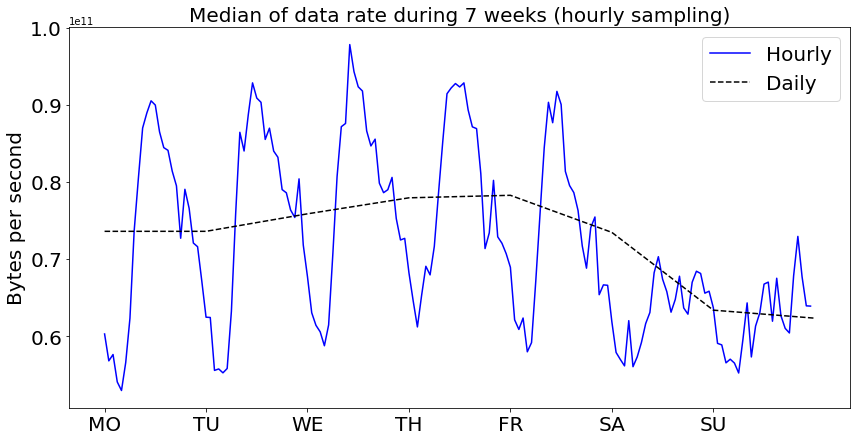
\includegraphics[width=\columnwidth]{img/BCH_byterate.png}
          \caption{Data-rate before new year holidays}
          \label{fig:BCH_bps}
    \end{subfigure}
    \begin{subfigure}{\figSzeMahdi\columnwidth}
          \centering
          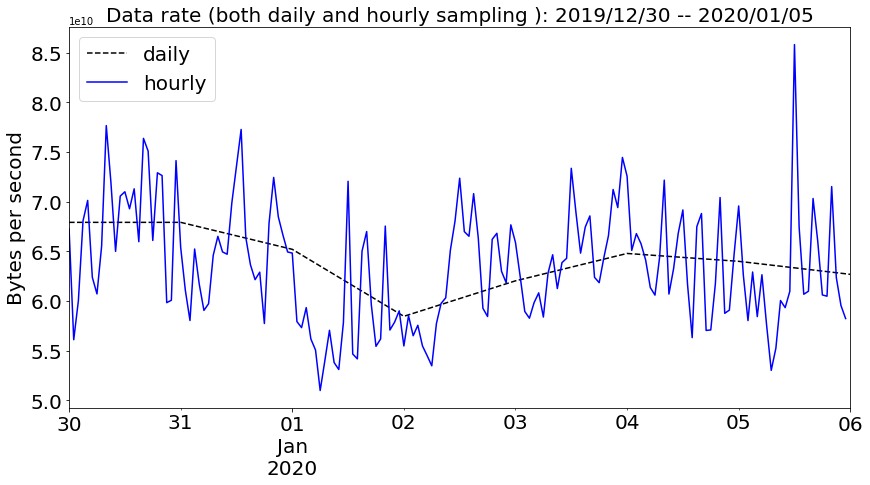
\includegraphics[width=\columnwidth]{img/CH2_byterate.png}
          \caption{Data-rate during new year holidays}
          \label{fig:CH_bps}
    \end{subfigure}
    \caption{Impact of new year holidays on data rate}
    \label{fig:datarate_BCH_CH}
\end{figure}
Fig.~\ref{fig:datarate_BCH_CH} show the impact of new year holidays on the total data rate throughput. There is an evident pattern during the week long before new year holidays. Total network throughput is between ~55 and ~110 Gbps during working days of ordinary week, however, it fluctuates between ~50 and ~80 Gbps during new year holidays. This means that data-rate had been reduced by ~30$\%$ during new year holidays excepting the weekend. Although the data-rate pattern at the weekend had a significant change, the overall data communicated during the weekend had not been changed significantly.

\begin{figure}[hbt!]
    \centering
    \begin{subfigure}{\figSzeMahdi\columnwidth}
          \centering
          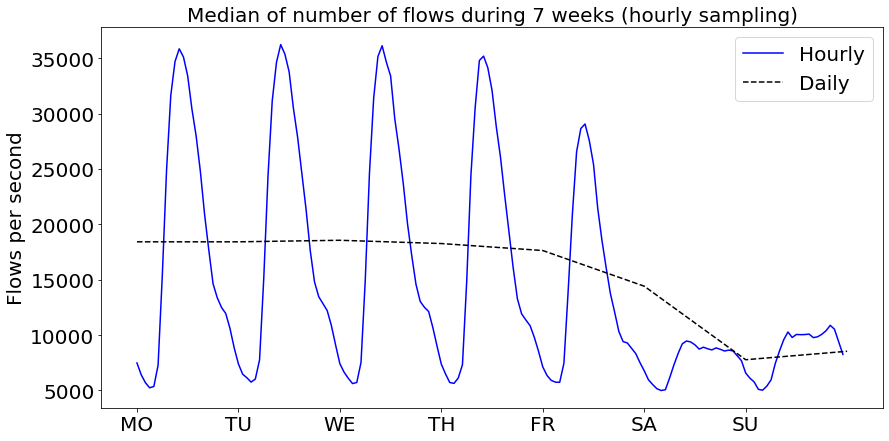
\includegraphics[width=\columnwidth]{img/BCH_flowrate.png}
          \caption{Flow-rate before new year holidays}
          \label{fig:BCH_fps}
    \end{subfigure}
    \begin{subfigure}{\figSzeMahdi\columnwidth}
          \centering
          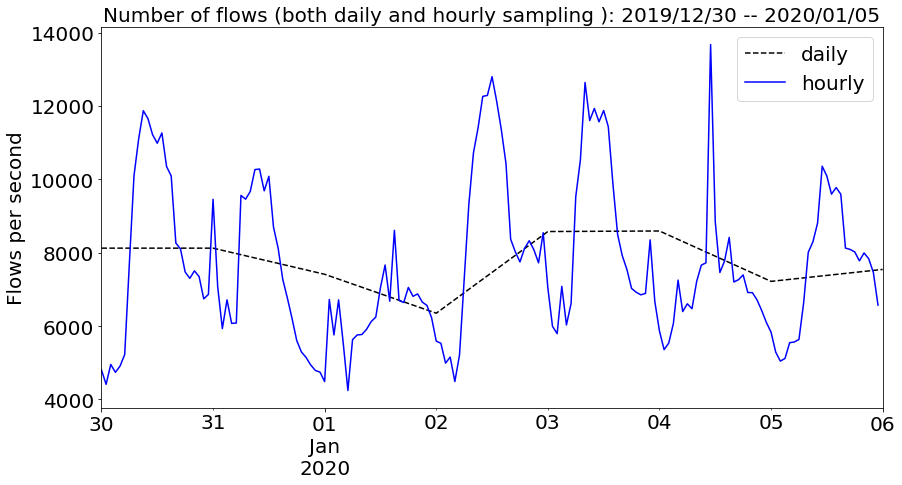
\includegraphics[width=\columnwidth]{img/CH2_flowrate.png}
          \caption{Flow-rate during new year holidays}
          \label{fig:CH_fps}
    \end{subfigure}
    \caption{Impact of new year holidays on flow rate}
    \label{fig:flowrate_BCH_CH}
\end{figure}
Fig.~\ref{fig:BCH_fps} illustrates network throughput in term of flow per second during the ordinary week and new year holidays. The number of flows per second traversing GEANT network infrastructure during ordinary working days is typically between 4.7~kfps and 40~kfps. The upper bound reduces to 15~kfps over the weekend.The number of flows traversing the network is highly related to the time-of-day and day-of-week. During the night, the network conveys the lowest number of flows. 
On the other hand, during the new year holidays the number of flows reduces notably and stays between 4~kfps and 14~kfps. Flow throughput on the day of new year not only has a significant reduction but also has a shift towards night-time usage (this is more clear in Fig.~\ref{fig:BCH_CH2_hourly_fps}). This shows that there are many new flows traversing GEANT network after mid-night of new year. The new flows enter the network after mid-night and leaves the network before 6am. On the new year day, the night-time flow throughput is comparable to day-light-time.

\begin{figure}
    \centering
    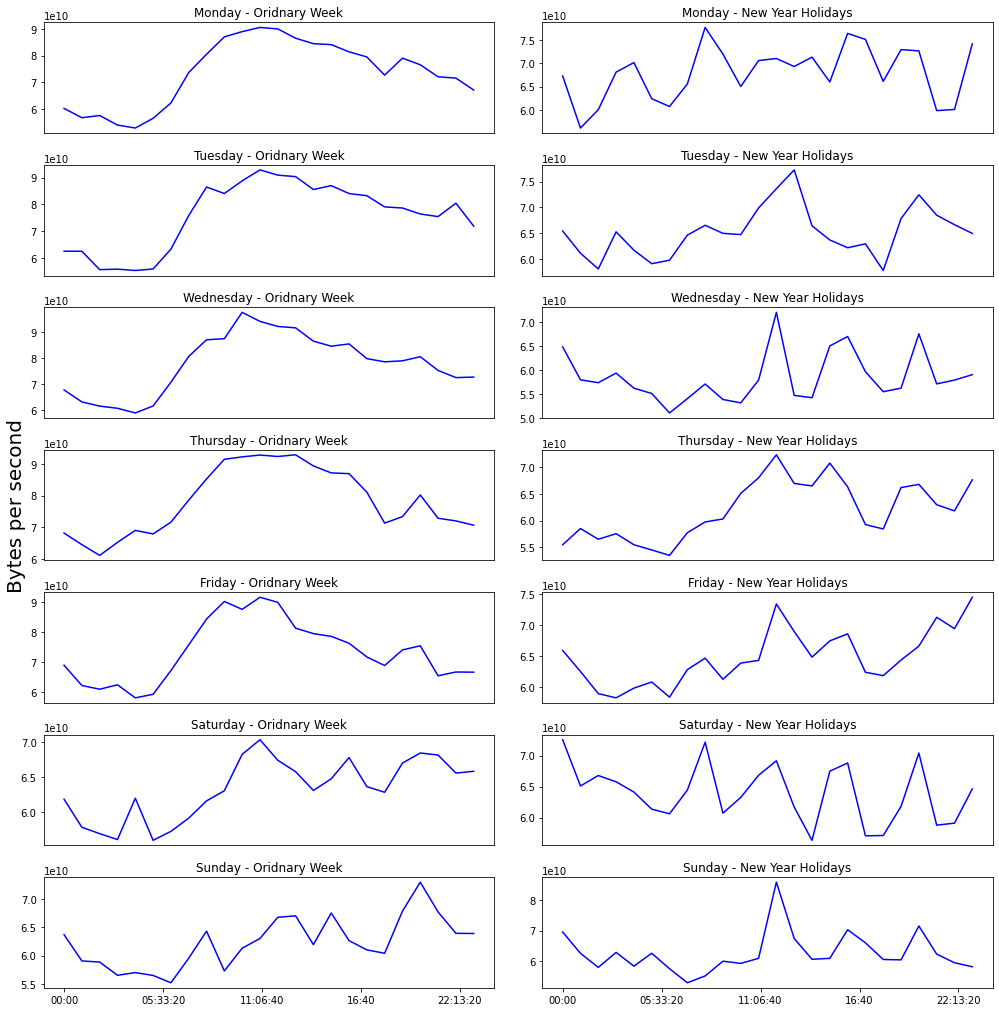
\includegraphics[width=\columnwidth]{img/BCH_CH2_hourly_compare_bps.png}
    \caption{Impact of new year holidays on traffic data-rate pattern}
    \label{fig:BCH_CH2_hourly_bps}
\end{figure}
In Fig.~\ref{fig:BCH_CH2_hourly_bps}, the impact of new year holidays on hourly pattern of data-rate during different days is investigated. There is an evident change of pattern during new year holidays. During ordinary working days, the data throughput is highly related to time-of-day and it shows a significant reduction after mid-night. The dependence to the time-of-day decreases during ordinary weekend, however, there is still a significant reduction at 4am. On the other hand, during new year holidays data-rate pattern is highly independent of time-of-day, especially during new year day and week-ends.

\begin{figure}
    \centering
    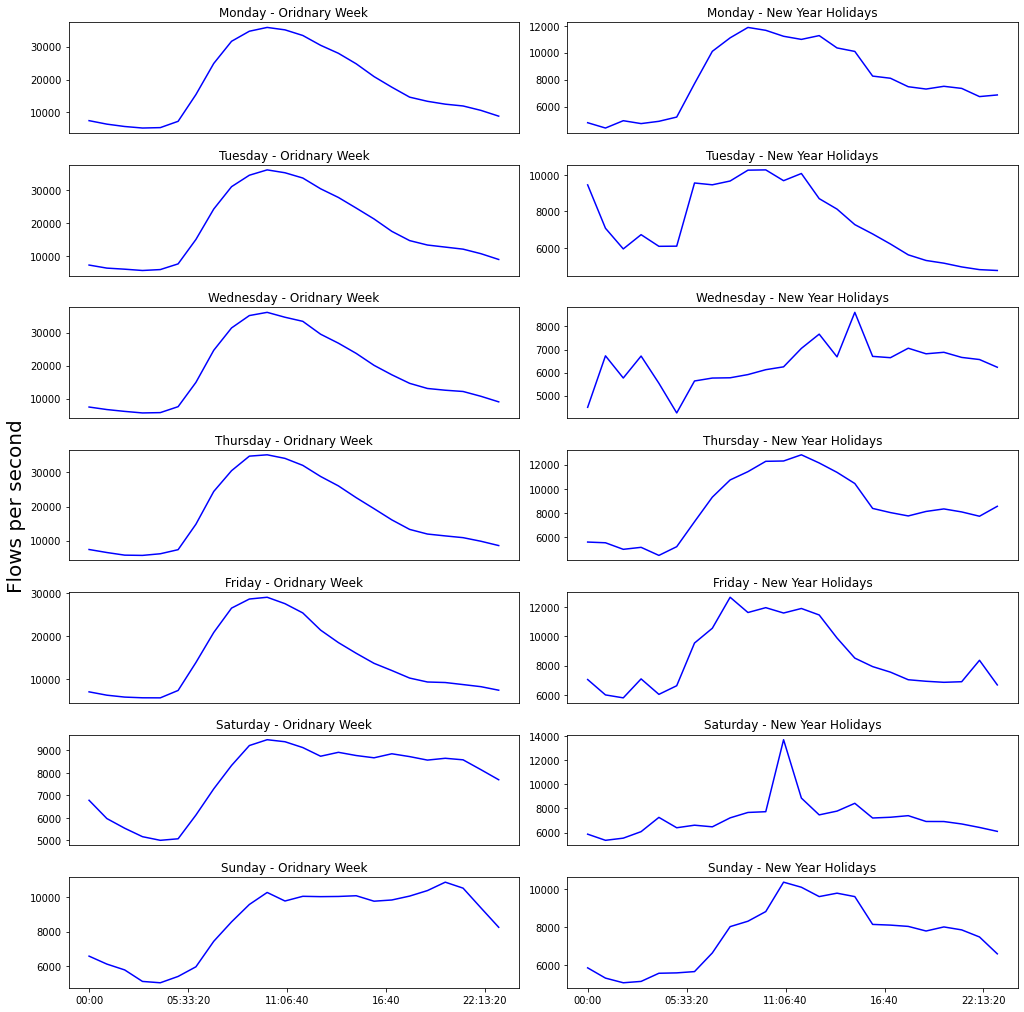
\includegraphics[width=\columnwidth]{img/BCH_CH2_hourly_compare_fps.png}
    \caption{Impact of new year holidays on traffic flow-rate pattern}
    \label{fig:BCH_CH2_hourly_fps}
\end{figure}
Fig.~\ref{fig:BCH_CH2_hourly_fps} compares the flow throughput pattern long before and during new year holidays. There is a clear pattern on the number of flows traversing the network on working days. Not only the pattern but also the upper and lower band is common during ordinary working days. Keeping the day of new year and the day before that, new year holidays mostly causes a significant reduction on the number of flows traversing the network but the pattern of flow throughput is almost the same as before. 

\subsection{Academic and Business Traffic}
In this part, we break down the traffic into its academic and business elements. To this end, we label the flows by their source and destination ASes. If an AS belongs to GEANT customer corn, it is considered as an academic AS, otherwise, it is considered as a business AS. For the sake of simplicity, in the following plots, if a flow is originated by an academic AS and destined to another academic AS we call it Academic-to-Academic (A2A) flow. Similarly, B2B, A2B, and B2A are abbreviations for Business-to-Business, Academic-to-Business, and Business-to-Academic flows, respectively.

\begin{figure}[hbt!]
    \centering
    \begin{subfigure}{\figSzeMahdi\columnwidth}
          \centering
          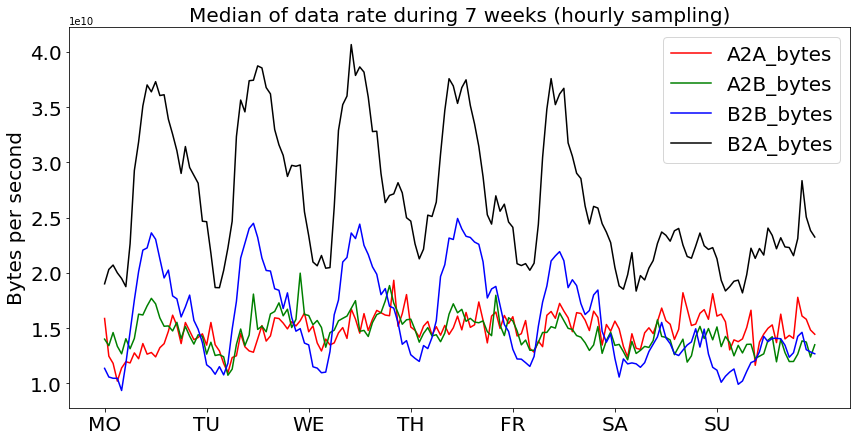
\includegraphics[width=\columnwidth]{img/BCH_acaBus_bps.png}
          \caption{Data-rate before new year holidays}
          \label{fig:BCH_acaBus_bps}
    \end{subfigure}
    \begin{subfigure}{\figSzeMahdi\columnwidth}
          \centering
          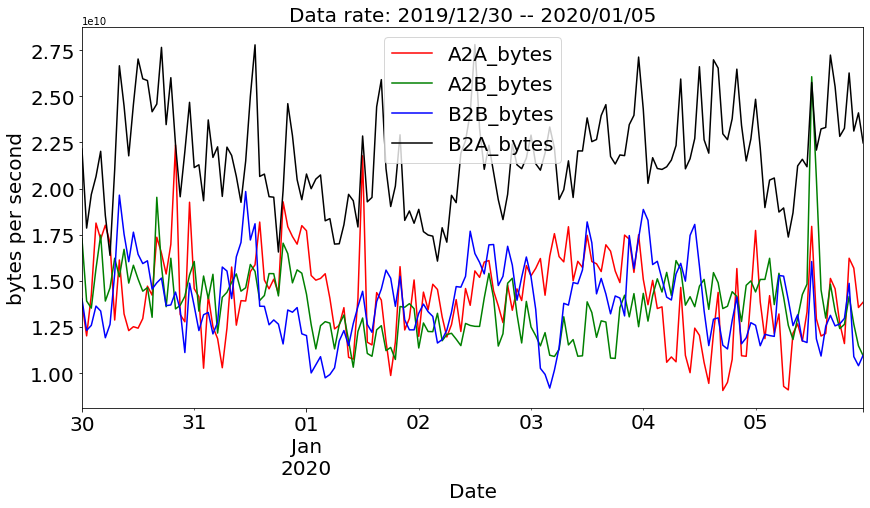
\includegraphics[width=\columnwidth]{img/CH2_acaBus_bps.png}
          \caption{Data-rate during new year holidays}
          \label{fig:CH_acaBus_bps}
    \end{subfigure}
    \caption{Impact of new year holidays on data rate of academic and business traffic}
    \label{fig:datarate_acaBus_BCH_CH}
\end{figure}
Fig.~\ref{fig:datarate_acaBus_BCH_CH} illustrates the data-rate pattern of Academic-to-Academic, Business-to-Business, Academic-to-Business, and Business-to-Academic traffic during an ordinary week and new year holidays. During working days, traffics originating from business ASes are more predictable comparing those originating from Academic ASes. This shows that 

\begin{figure}[hbt!]
    \centering
    \begin{subfigure}{\figSzeMahdi\columnwidth}
          \centering
          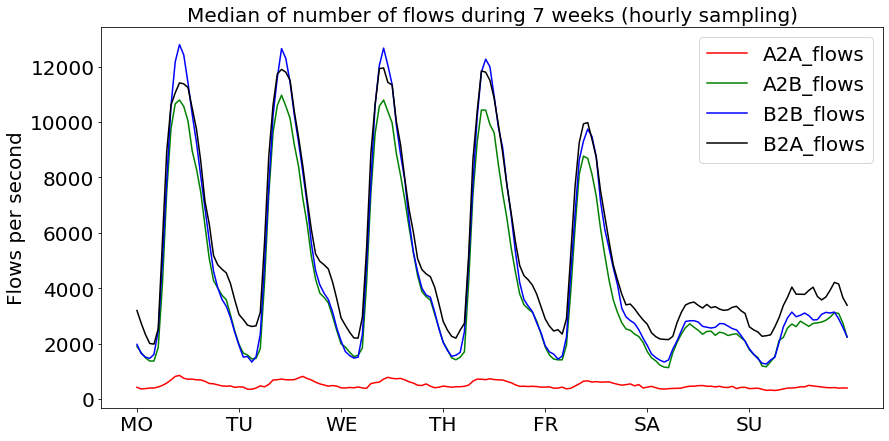
\includegraphics[width=\columnwidth]{img/BCH_acaBus_fps.png}
          \caption{Flow-rate before new year holidays}
          \label{fig:BCH_acaBus_fps}
    \end{subfigure}
    \begin{subfigure}{\figSzeMahdi\columnwidth}
          \centering
          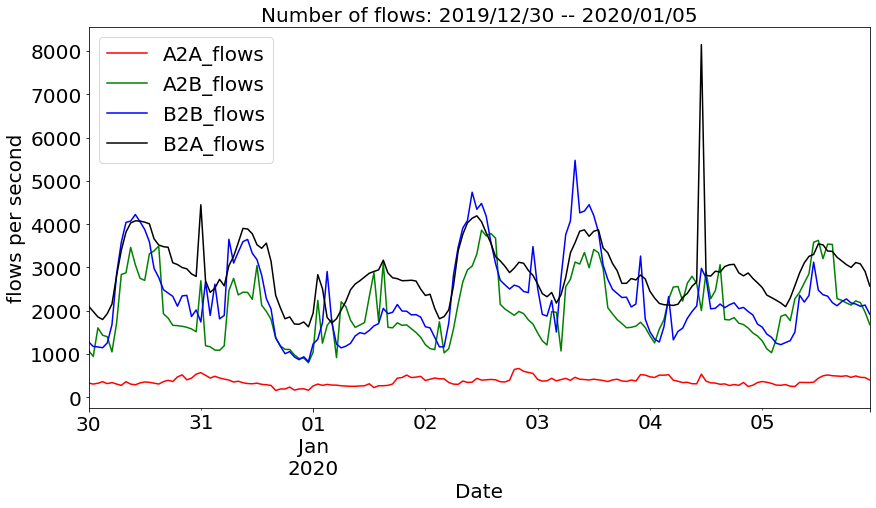
\includegraphics[width=\columnwidth]{img/CH2_acaBus_fps.png}
          \caption{Flow-rate during new year holidays}
          \label{fig:CH_acaBus_fps}
    \end{subfigure}
    \caption{Impact of new year holidays on flow rate of academic and business traffic}
    \label{fig:flowrate_acaBus_BCH_CH}
\end{figure}

\subsection{NRENs Traffic}

\subsection{Top ASes}
\begin{figure}[hbt!]
    \centering
    \begin{subfigure}{\columnwidth}
          \centering
          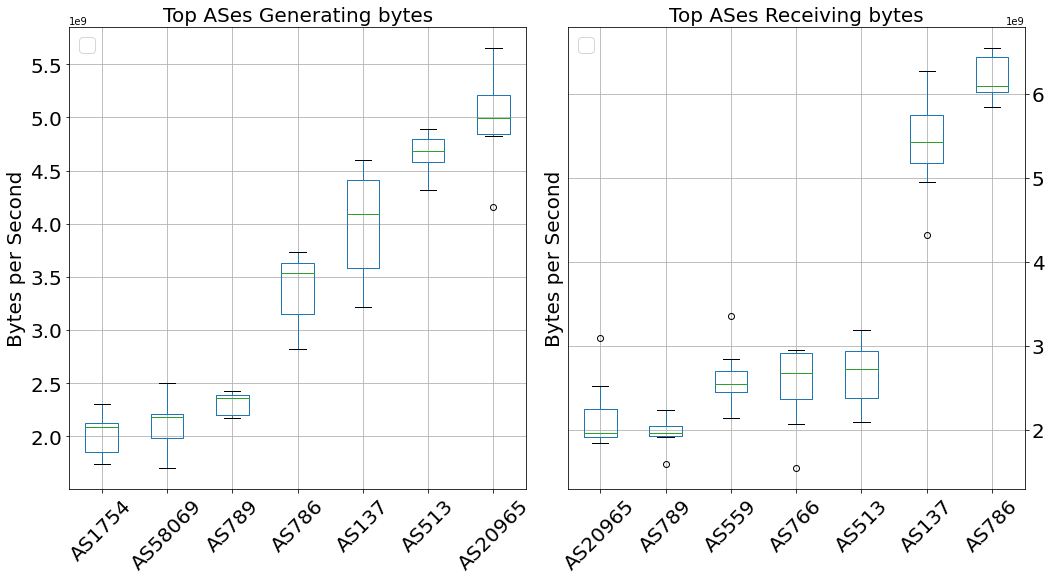
\includegraphics[width=\columnwidth]{img/OWBCH_top7ASes_bps.png}
          \caption{Data-rate before new year holidays}
          \label{fig:OWBCH_topAS_bps}
    \end{subfigure}
    \begin{subfigure}{\columnwidth}
          \centering
          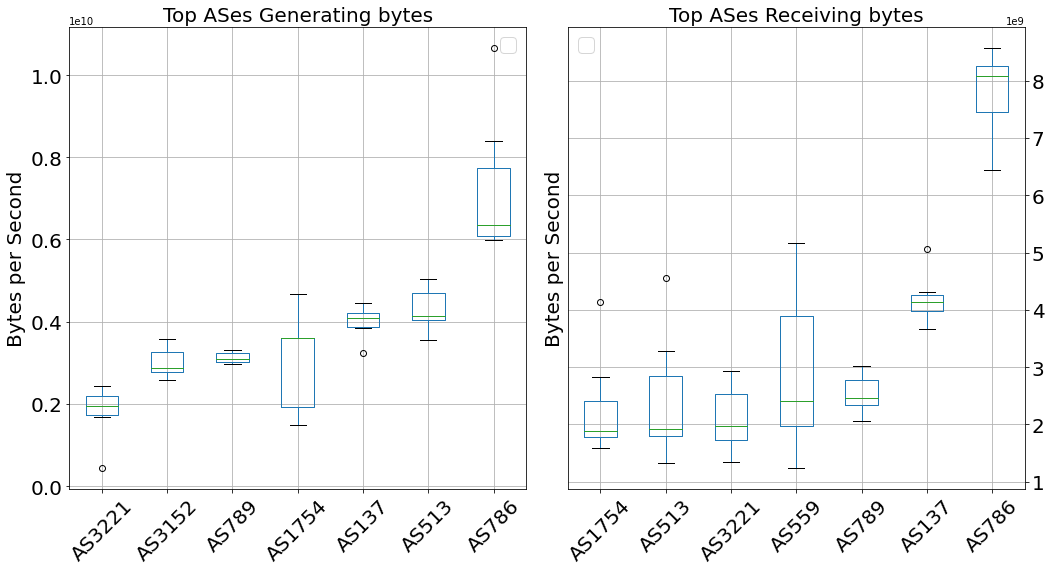
\includegraphics[width=\columnwidth]{img/CH2_top7ASes_bps.png}
          \caption{Data-rate during new year holidays}
          \label{fig:CH_topAS_bps}
    \end{subfigure}
    \caption{Impact of new year holidays on data-rate of top 7 ASes}
    \label{fig:topAS_bps_OW_CH}
\end{figure}

\begin{figure}[hbt!]
    \centering
    \begin{subfigure}{\columnwidth}
          \centering
          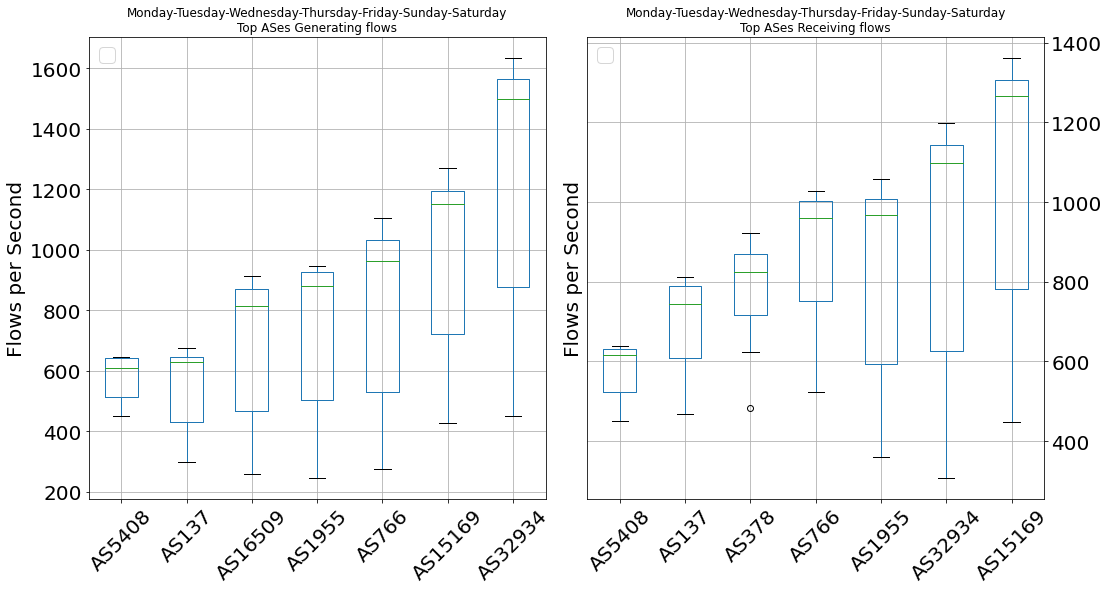
\includegraphics[width=\columnwidth]{img/OWBCH_top7ASes_fps.png}
          \caption{Data-rate before new year holidays}
          \label{fig:OWBCH_topAS_fps}
    \end{subfigure}
    \begin{subfigure}{\columnwidth}
          \centering
          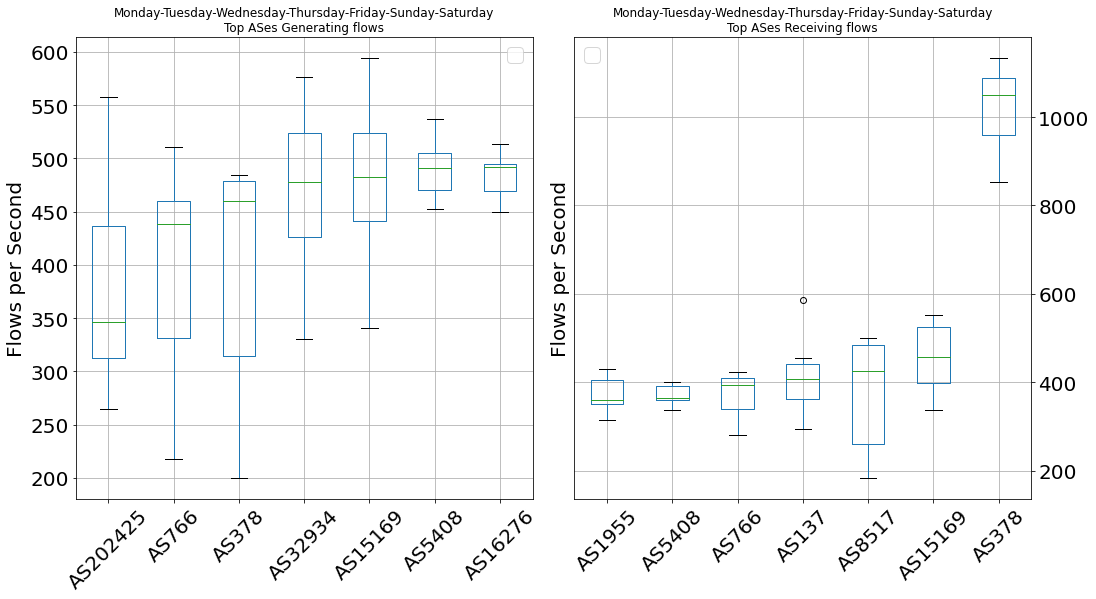
\includegraphics[width=\columnwidth]{img/CH2_top7ASes_fps.png}
          \caption{Data-rate during new year holidays}
          \label{fig:CH_topAS_fps}
    \end{subfigure}
    \caption{Impact of new year holidays on flow-rate of top 7 ASes}
    \label{fig:topAS_fps_OW_CH}
\end{figure}



\subsection{Discussion}



\section{Impact of Covid-19 on GEANT}
In this section, we look into the impact of 'Covid-19 pandemic' on GEANT traffic pattern. To this end, we do sampling over two different time-periods, one in January-February-March before Covid-19 pandemic in Europe (2020/01/20 - 2020/03/15) and the other one during the pandemic (2020/03/16 - 2020/03/22). In order to be able to compare these two periods, the data sampled during 2020/01/20-2020/03/15 has been mapped to a one week period by considering the median of values observed during similar 'day of week' and 'time of day'. For the sake of simplicity, we refer to this period as ordinary week before Covid-19 pandemic. We first analyse the total traffic throughput in terms of byte per second (bps) and flow per second (fps). Thereafter, we break-down the traffic into its academic and business elements and their pattern during the week. After that, the top NRENs generating and receiving traffic is discussed to investigate the impact of Covid-19 pandemic on top NRENs pattern. The same story is built for top ASes generating and receiving traffic.

\subsection{Total Traffic Throughput}
Due to the COVID19 pandemic, traffic in terms of bytes dropped by almost one-third, whereas overall flows dropped by almost half. This difference in observation could be due to the nature of flows. A flow is a unidirectional sequence of packets that contains among other things an ingress interface, IP protocol, source and destination IP addresses, source and destination ports and type of service. While flows require an ingress interface and a request initiating a flow, traffic in bytes may just be machine-to-machine. This is further supported by similar trends during the Christmas/NYE holidays.

\begin{figure}[hbt!]
    \centering
    \begin{subfigure}{\figSzeMahdi\columnwidth}
          \centering
          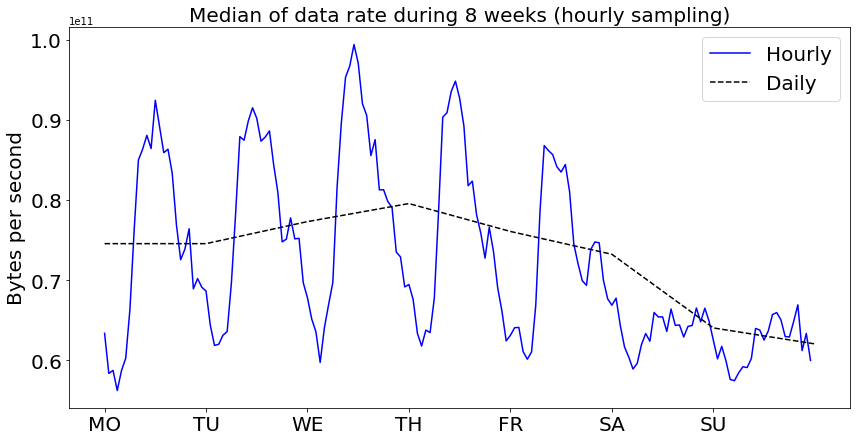
\includegraphics[width=\columnwidth]{img/BCO_byterate.png}
          \caption{Data-rate before COVID-19 pandemic}
          \label{fig:BCO_bps}
    \end{subfigure}
    \begin{subfigure}{\figSzeMahdi\columnwidth}
          \centering
          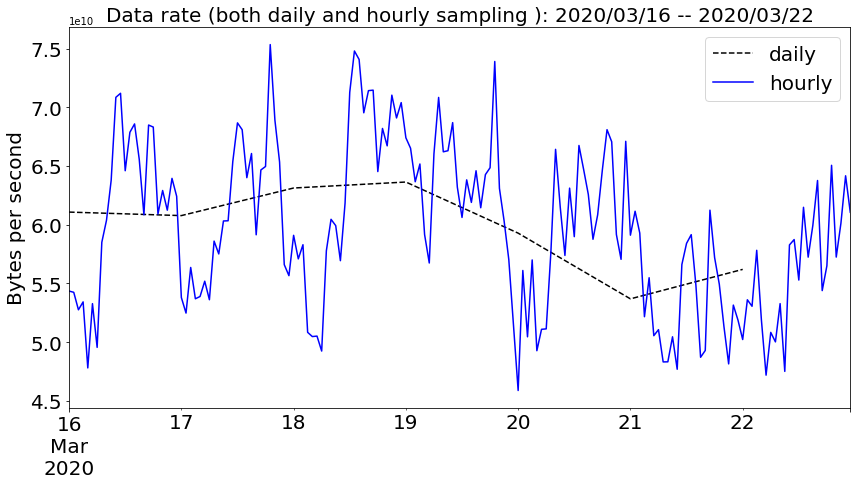
\includegraphics[width=\columnwidth]{img/CO2_byterate.png}
          \caption{Data-rate during COVID-19 pandemic}
          \label{fig:CO_bps}
    \end{subfigure}
    \caption{Impact of COVID-19 pandemic on data rate}
    \label{fig:datarate_BCO_CO}
\end{figure}

\begin{figure}
    \begin{subfigure}{\figSzeMahdi\columnwidth}
          \centering
          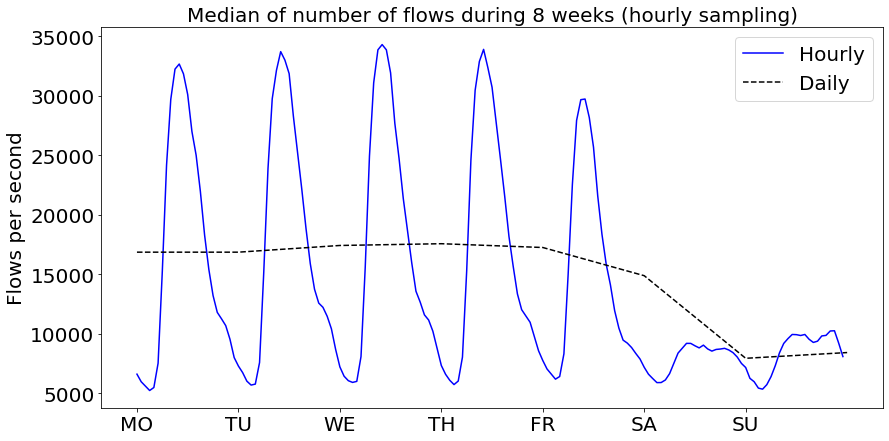
\includegraphics[width=\columnwidth]{img/BCO_flowrate.png}
          \caption{Flow-rate before COVID-19 pandemic}
          \label{fig:BCO_fps}
    \end{subfigure}
    \begin{subfigure}{\figSzeMahdi\columnwidth}
          \centering
          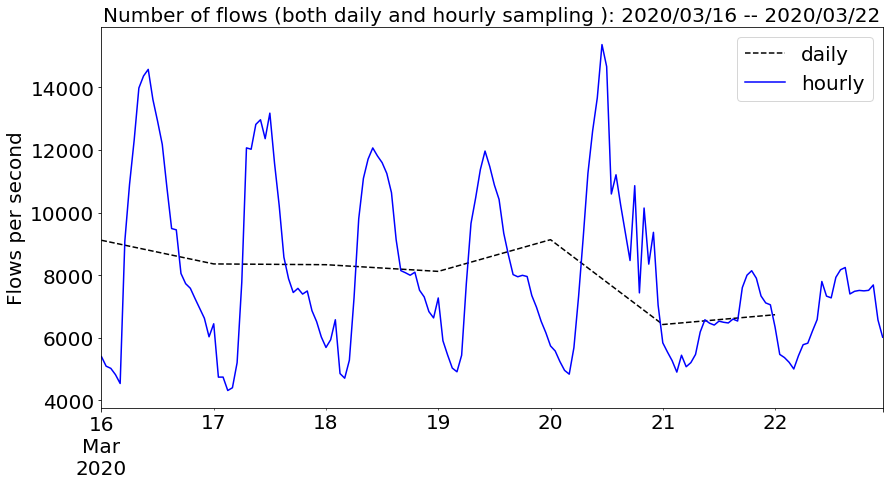
\includegraphics[width=\columnwidth]{img/CO2_flowrate.png}
          \caption{Flow-rate during COVID-19 pandemic}
          \label{fig:CO_fps}
    \end{subfigure}
    \caption{Impact of COVID-19 pandemic on flow rate}
    \label{fig:flowrate_BCO_CO}
\end{figure}

\subsection{Academic and Business Traffic}
\begin{figure}
    \begin{subfigure}{\figSzeMahdi\columnwidth}
          \centering
          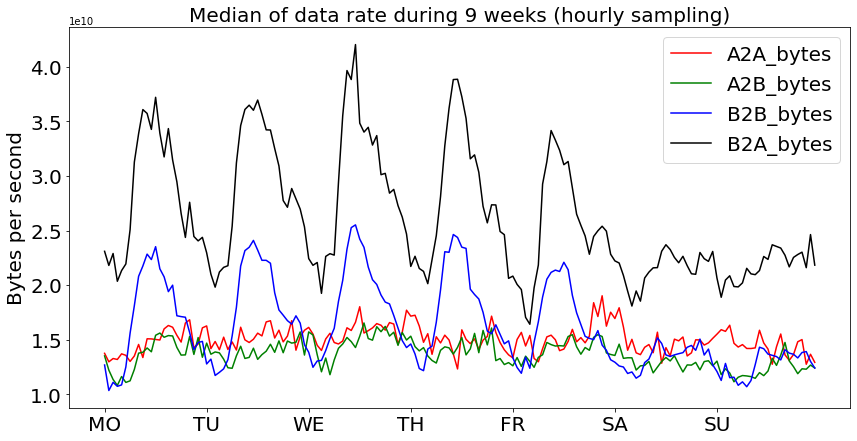
\includegraphics[width=\columnwidth]{img/BCO_acaBus_bps.png}
          \caption{Data-rate before COVID-19 pandemic}
          \label{fig:BCO_acaBus_bps}
    \end{subfigure}
    \begin{subfigure}{\figSzeMahdi\columnwidth}
          \centering
          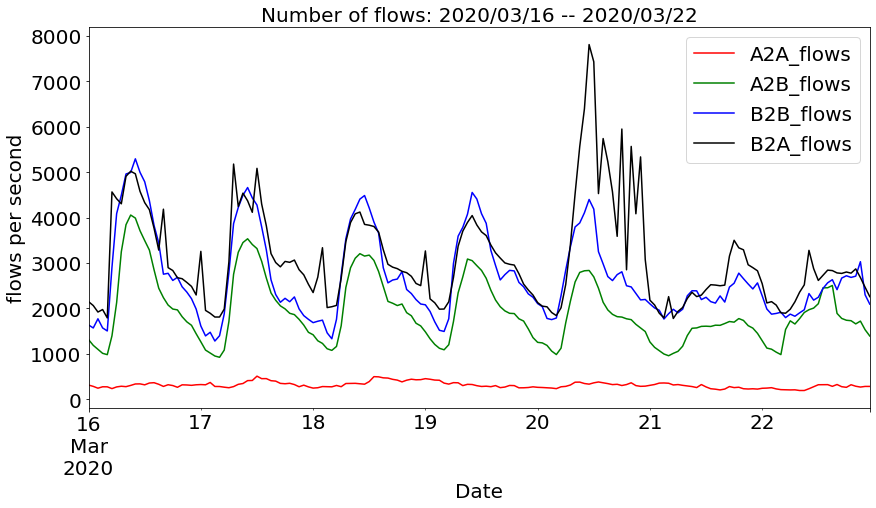
\includegraphics[width=\columnwidth]{img/CO2_acaBus_bps.png}
          \caption{Data-rate during COVID-19 pandemic}
          \label{fig:CO_acaBus_bps}
    \end{subfigure}
    \caption{Impact of COVID-19 pandemic on data rate of academic and business traffic}
    \label{fig:datarate_acaBus_BCO_CO}
\end{figure}

\begin{figure}
    \begin{subfigure}{\figSzeMahdi\columnwidth}
          \centering
          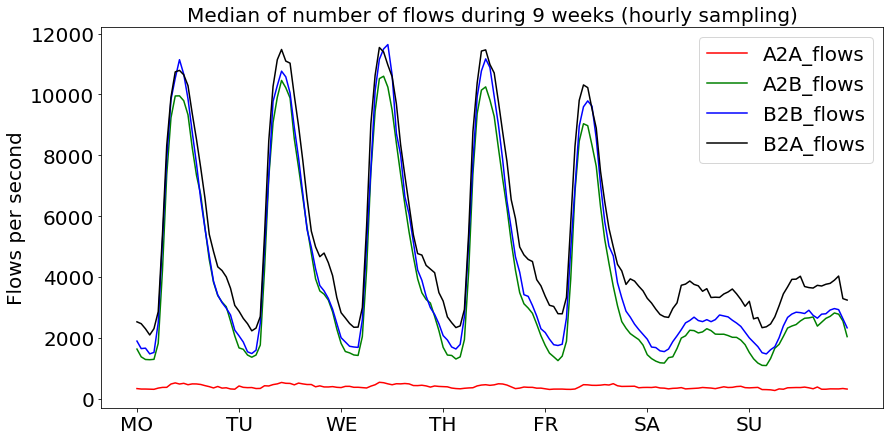
\includegraphics[width=\columnwidth]{img/BCO_acaBus_fps.png}
          \caption{Flow-rate before COVID-19 pandemic}
          \label{fig:BCO_acaBus_fps}
    \end{subfigure}
    \begin{subfigure}{\figSzeMahdi\columnwidth}
          \centering
          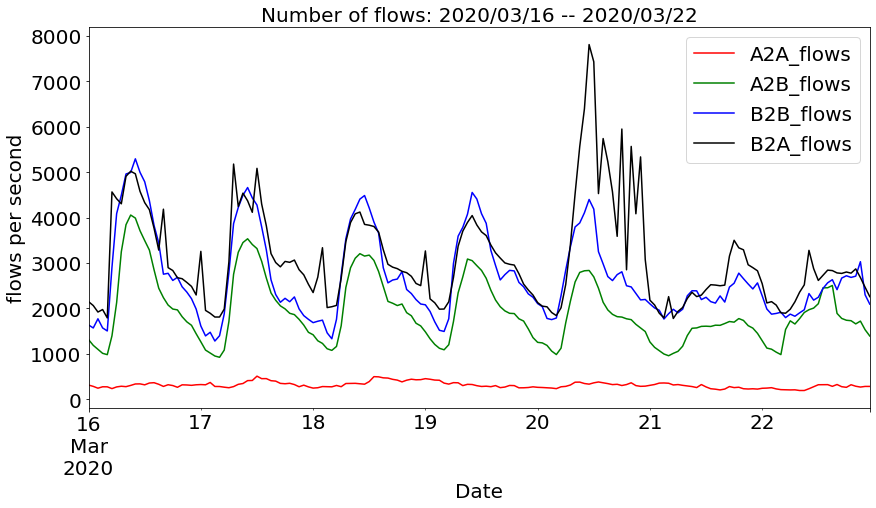
\includegraphics[width=\columnwidth]{img/CO2_acaBus_fps.png}
          \caption{Flow-rate during COVID-19 pandemic}
          \label{fig:CO_acaBus_fps}
    \end{subfigure}
    \caption{Impact of COVID-19 pandemic on flow rate of top ASes}
    \label{fig:flowrate_acaBus_BCO_CO}
\end{figure}
\subsection{NRENs Traffic}

\subsection{Top ASes}
\begin{figure}[hbt!]
    \centering
    \begin{subfigure}{\columnwidth}
          \centering
          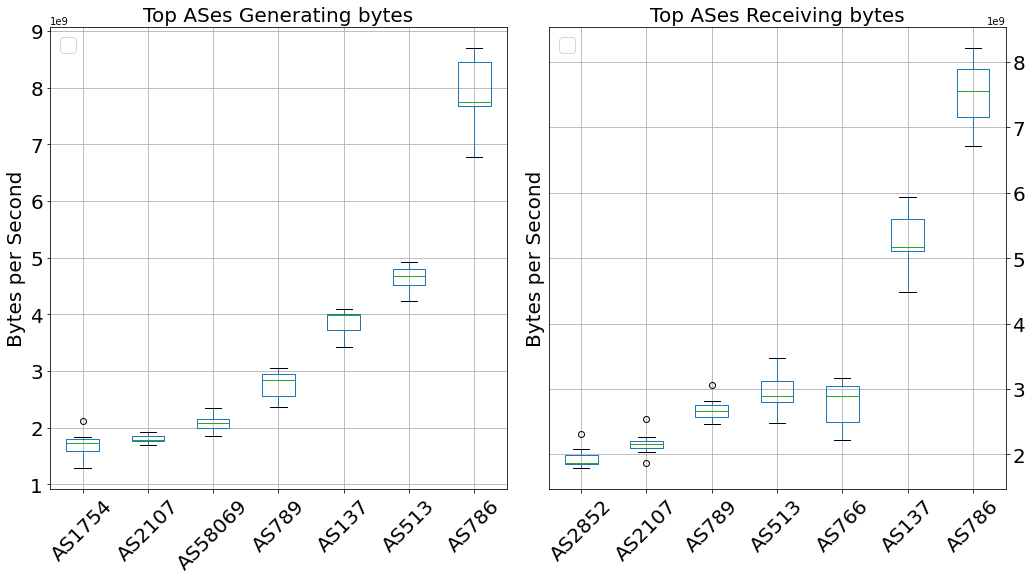
\includegraphics[width=\columnwidth]{img/OWBCO_top7ASes_bps.png}
          \caption{Data-rate before COVID-19 pandemic}
          \label{fig:OWBCO_topAS_bps}
    \end{subfigure}
    \begin{subfigure}{\columnwidth}
          \centering
          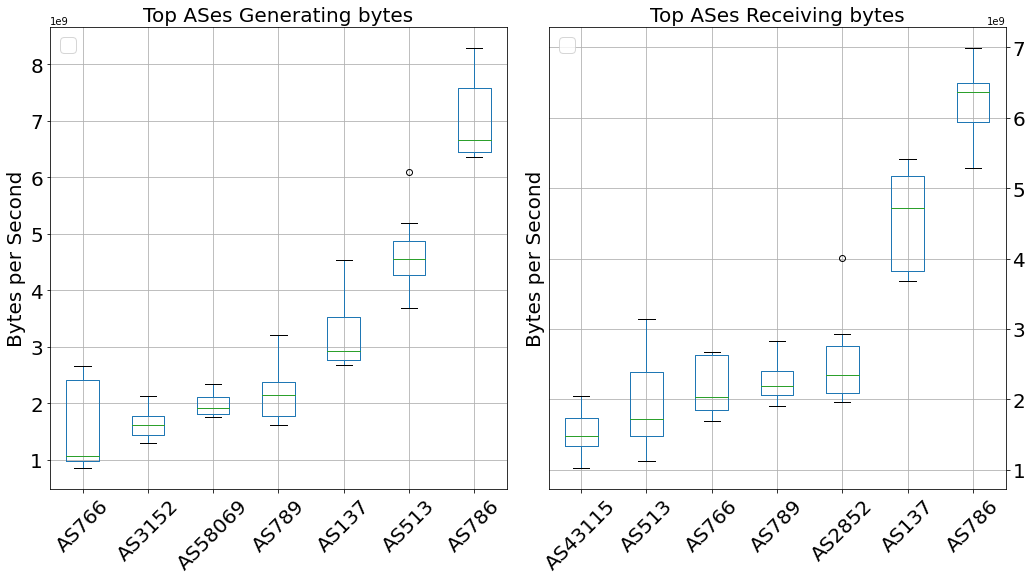
\includegraphics[width=\columnwidth]{img/CO2_top7ASes_bps.png}
          \caption{Data-rate during COVID-19 pandemic}
          \label{fig:CO_topAS_bps}
    \end{subfigure}
    \caption{Impact of COVID-19 pandemic on data-rate of top 7 ASes}
    \label{fig:topAS_bps_OW_CO}
\end{figure}

\begin{figure}[hbt!]
    \centering
    \begin{subfigure}{\columnwidth}
          \centering
          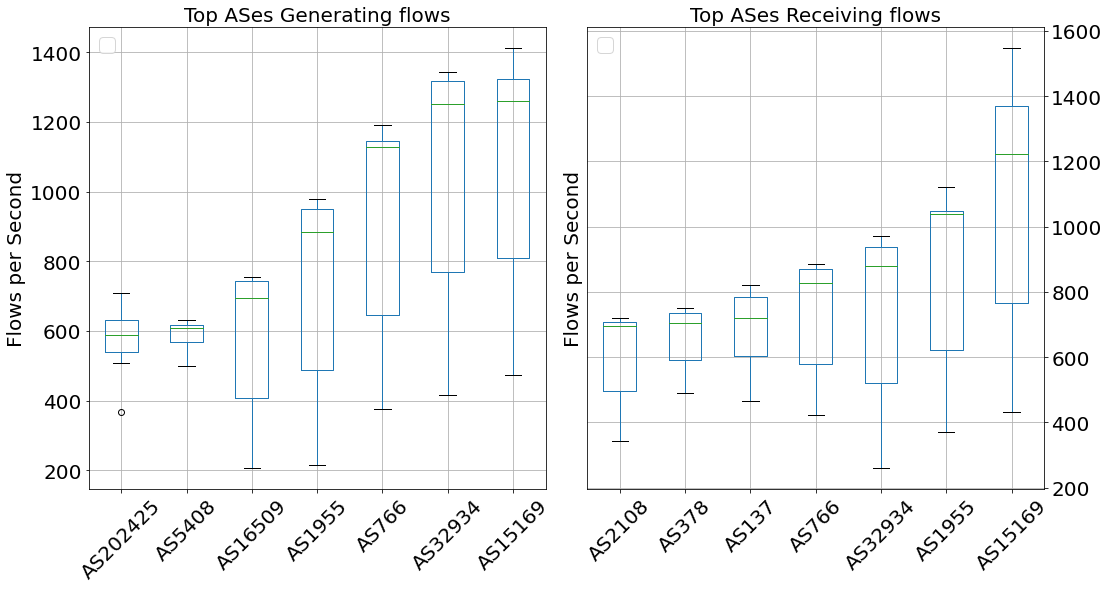
\includegraphics[width=\columnwidth]{img/OWBCO_top7ASes_fps.png}
          \caption{Data-rate before COVID-19 pandemic}
          \label{fig:OWBCO_topAS_fps}
    \end{subfigure}
    \begin{subfigure}{\columnwidth}
          \centering
          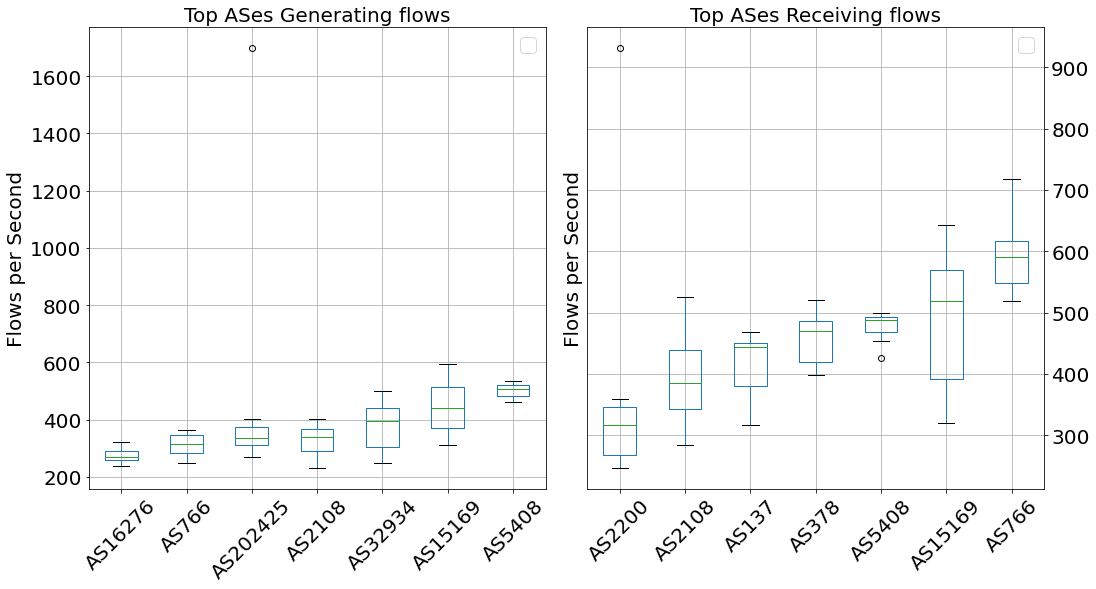
\includegraphics[width=\columnwidth]{img/CO2_top7ASes_fps.png}
          \caption{Data-rate during COVID-19 pandemic}
          \label{fig:CO_topAS_fps}
    \end{subfigure}
    \caption{Impact of COVID-19 pandemic on flow-rate of top 7 ASes}
    \label{fig:topAS_fps_OW_CO}
\end{figure}

\subsection{Discussion}

\section{Comparing Covid-19 and New Year Holidays impact on GEANT}




\section{OLD PARTS}
\subsection{Sankey Plot}
In these plots, the top-n one-way communications are considered. For example, consider

A->B: 10 bps (meaning that there is a traffic flow of 10 bps from A to B)
A->C: 1 bps
A->D: 9bps
B->C:11bps
B->D: 3bps
B->A:5bps
then the top-3 one-way communications are:
A->B:10bps
A-D:9bps
B-C:11bps

AS-Level Analysis: every AS is considered as a unique entity. Each NREN has one or more AS-number. Each of these numbers are considered as one unique entity.

NREN-Level Analysis: all ASes belonging to an NREN are aggregated together, e.g., consider AS7 is in customer cone of AS786 (JISC). The traffic generated by AS7 and destinated to AS-x (AS7 -> AS-x) will be considered as AS786 -> AS-x. Besides, if there are more than one ASN assigned to an NREN, these ASNes would be aggregated into one, e.g., if AS786 and AS133084 are both assigned to JISC then we replace AS133084 with AS786 everywhere.



\subsection{ASes}

\red{For top ASes we will need to know the overlap (i.e. common ASes) for measurement criteria. That is, how many top ASes in terms of generating traffic measured in bps are in the top ASes list if measured in terms of fps. And vice versa, e.g. receiving traffic in bps and fps, etc.}

\subsubsection{Top ASes fps and bps (box plot)}
In the following, top ASes are specified. The approach used to specify the top ASes is 'top over time': average the total output of each AS during the sampling period, and select the top x ASes.
Each AS may generate traffic or receives traffic, therefore, plots are divided into two categories 'Top ASes Generating Traffic' and 'Top ASes Receiving Traffic'.

\end{document}
